\section{实验设计与结果}
\label{sec:results}
\subsection{匿名化效果}
匿名化围绕面部内部的外观变化与区域保持进行观察。图\ref{fig:anon}给出同一来源样本处理前后的对照：面部纹理和局部五官外观发生改变，周围头发与背景保留在原位置，眼睛开合与嘴部形态仍可辨认。图中各组均由输入经过匿名处理得到，不依据原图预测类别挑选另一张表情图片。

\begin{figure}[htbp]
\centering
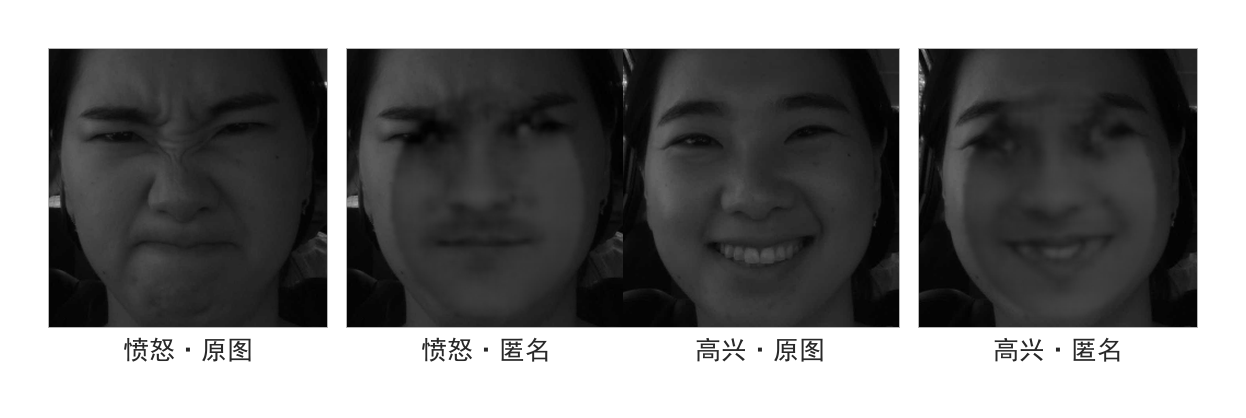
\includegraphics[width=\linewidth]{anonymization_best_sheet.png}
\caption{局部人脸匿名化的原图与结果对照}
\label{fig:anon}
\end{figure}

项目内身份评价以自建 IdentityNet 为对象，先固定面部裁剪范围与归一化方式，再对原脸和匿名脸分别预测。评价重点是匿名后能否继续命中原身份，同时观察特征相似程度和面部外像素保持情况。身份模型只承担离线比较，不参与表情类别选择，也不进入实时业务链路。

\begin{table}[htbp]
\centering
\caption{匿名化评价的项目内比较方式}
\label{tab:privacy}
\begin{tabularx}{\linewidth}{@{}lXX@{}}
\toprule
比较项 & 比较方式 & 评价作用\\
\midrule
原身份命中 & 固定自建身份模型，比较原脸与匿名脸 & 衡量原身份关联是否被削弱\\
面部变化 & 对照五官、纹理及脸部局部结构 & 观察匿名外观变化\\
区域保持 & 比较合成掩膜外灰度像素 & 核对头发与背景保持\\
表情可用性 & 匿名脸与真实表情标签比较 & 检查下游识别任务\\
\bottomrule
\end{tabularx}
\end{table}

\subsection{表情识别}
表\ref{tab:expression}使用主分支保存的分域统计，全部表情输入均为匿名灰度脸。表中实时基线作为质量配置的对照记录。PPB-Emo 两个集合统计中性样本，KMU-FED 统计六类座舱样本，RAF-DB 统计七类自然场景样本。

\begin{table}[htbp]
\centering
\caption{匿名灰度输入的分域表情识别结果}
\label{tab:expression}
\begin{tabular}{@{}llrr@{}}
\toprule
配置 & 验证集合 & 样本数 & 准确率\\
\midrule
实时基线 & RAF-DB 验证 & 3\,068 & 60.50\%\\
实时基线 & KMU-FED 尾帧 & 220 & 99.09\%\\
实时基线 & PPB-Emo 验证 & 34 & 91.18\%\\
实时基线 & PPB-Emo 测试 & 35 & 100.00\%\\
\midrule
质量 & RAF-DB 验证 & 3\,068 & 78.39\%\\
质量 & KMU-FED 尾帧 & 220 & 99.55\%\\
质量 & PPB-Emo 验证 & 34 & 100.00\%\\
质量 & PPB-Emo 测试 & 35 & 100.00\%\\
\bottomrule
\end{tabular}
\end{table}

质量配置在 RAF-DB 上比表中实时对照提高 17.89 个百分点，在 KMU-FED 上正确识别 219 张，在 PPB-Emo 中性验证和测试中分别正确识别 34 张与 35 张。按真实标签统计而非单帧置信度评价，可以直接观察匿名输入是否仍能支持表情分类。

\begin{figure}[htbp]
\centering
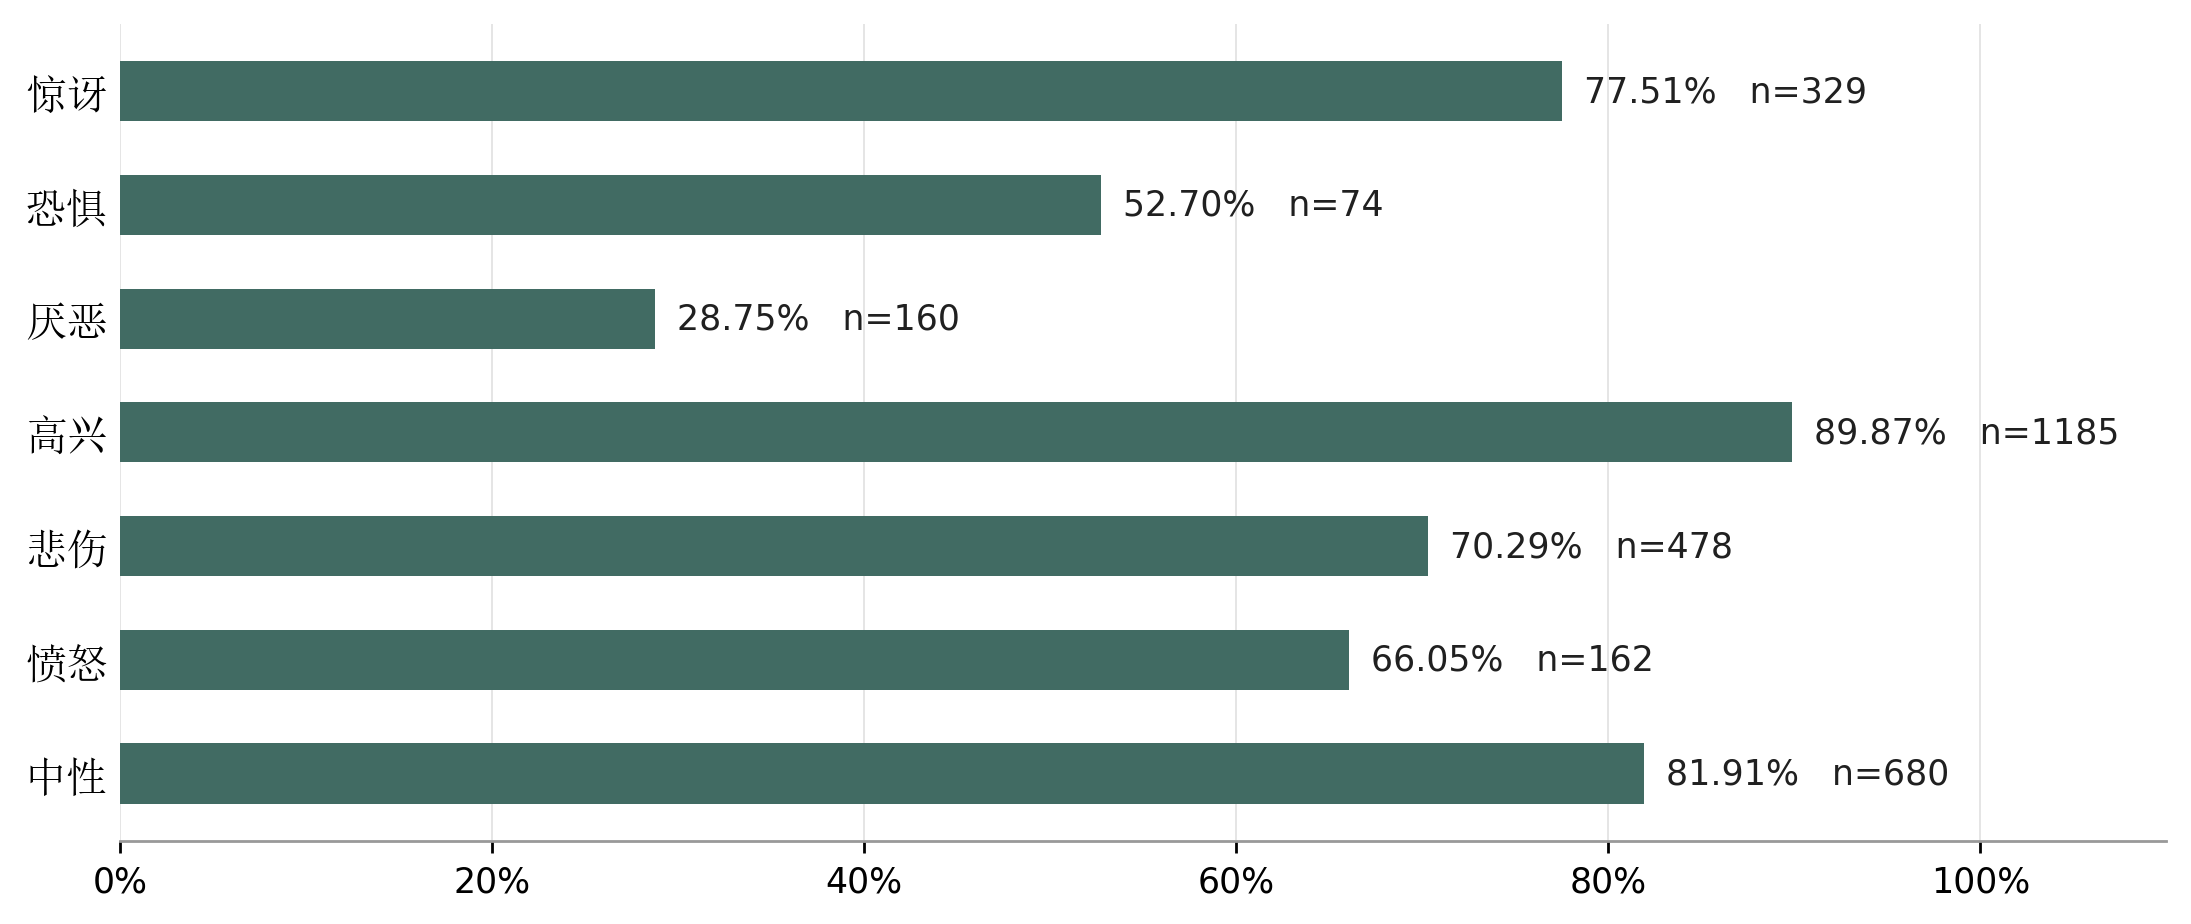
\includegraphics[width=.86\linewidth]{expression_metrics.png}
\caption{质量配置的 RAF-DB 七类表情召回率}
\label{fig:class}
\end{figure}

图\ref{fig:class}按真实类别统计，RAF-DB 中高兴类召回率为 89.87\%，中性类为 81.91\%，惊讶类为 77.51\%。中性召回对应 680 张中性图像中的 557 张正确预测，为座舱常见静态表情提供了明确的观察指标。各数据集保留各自的标签与划分口径，便于复现和对比。

\subsection{实时性能与桌面端}
长视频记录中，高速运行的稳态分析速度为 29.13--33.99 FPS，测量包含匿名化和表情分析的模型处理时间。该结果对应连续视频中的稳态区间，模型加载、质量配置和输出编码另行计时；桌面刷新速度不代替分析帧率。

图片实验页将带真实标签的样本列表、原始灰度图与匿名图集中展示，用户可逐张比较匿名外观、表情预测和置信度。图\ref{fig:ui}为桌面端实际运行画面。

\begin{figure}[htbp]
\centering
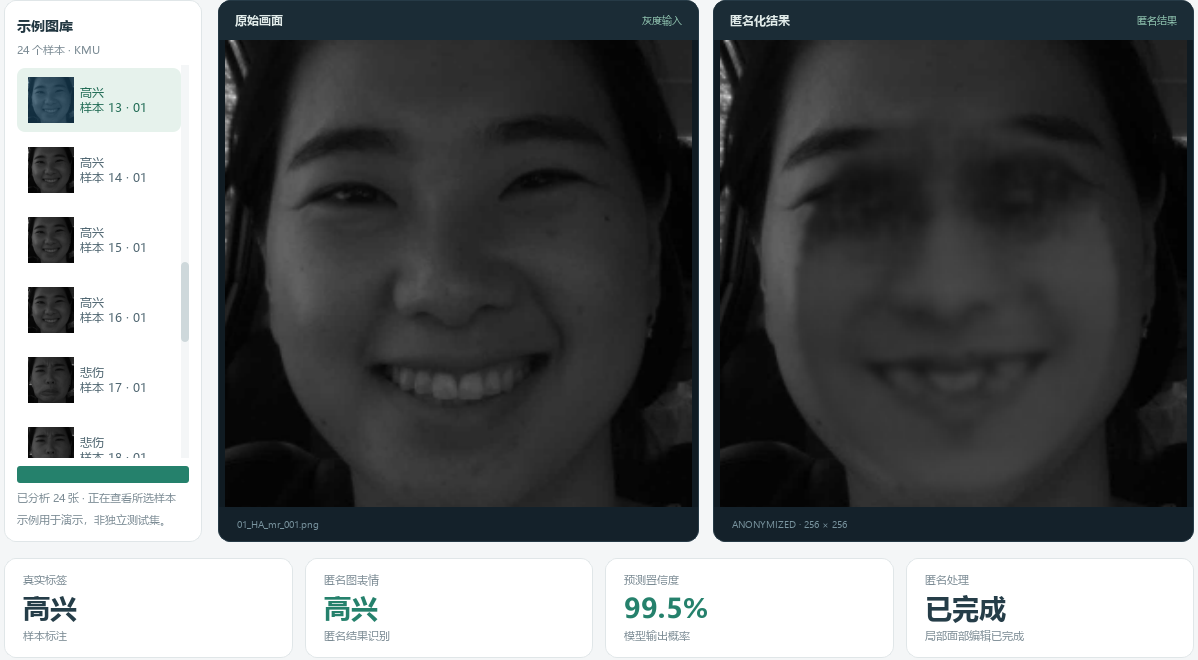
\includegraphics[width=\linewidth]{ui_image_detail.png}
\caption{桌面图片实验：真实标签、匿名对照与表情结果}
\label{fig:ui}
\end{figure}

实时页支持摄像头、本地视频和示例视频，并提供高速、质量两种选择。画面同步显示原始灰度输入与匿名输出，结果面板显示匿名图表情、置信度、当前分析帧和模型 FPS。视频停止或切换来源时释放旧任务，避免上一段视频结果混入当前画面。

\begin{figure}[htbp]
\centering
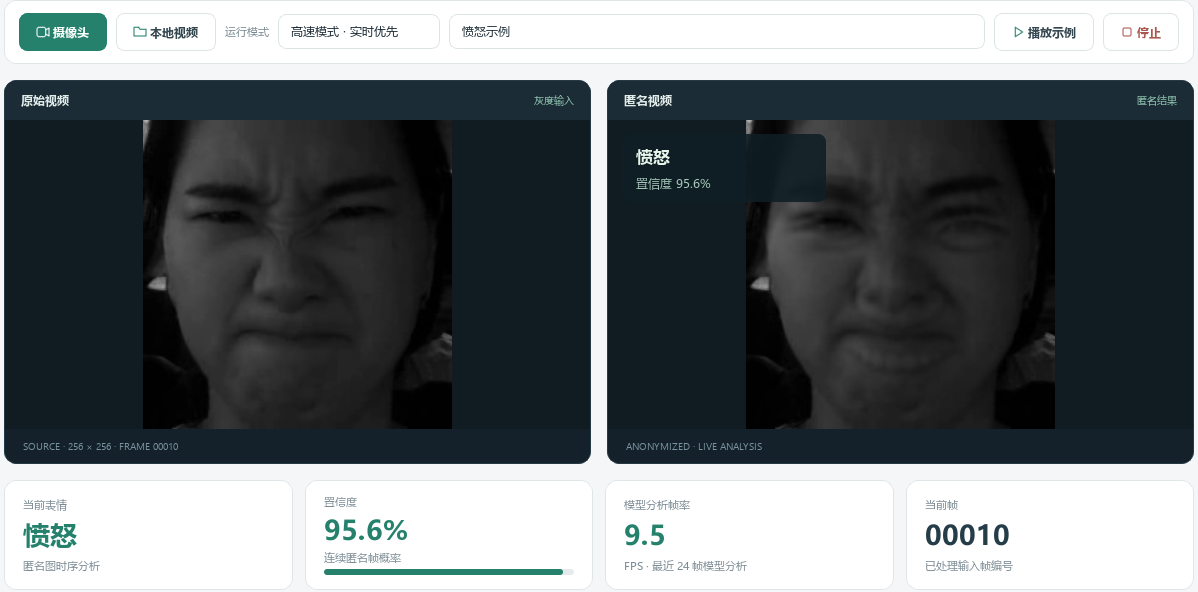
\includegraphics[width=\linewidth]{ui_video_detail.png}
\caption{实时分析：匿名视频上的表情与置信度}
\label{fig:uivideo}
\end{figure}

模型表现页集中呈现按数据集划分的准确率、样本量和类别统计，与图片实验页的单张输出形成互补。三页分别服务于样本检查、连续演示和整体评价，使系统的处理过程与结果可以直观对应。
